\apendice{Especificación de diseño}

\section{Introducción}

La especificación de diseño es un componente fundamental en la creación de sistemas robustos y escalables. En esta sección se detallará el diseño de los datos, secuencias y arquitectura del \textit{software} desarrollado. Esto permite visualizar de forma sencilla la estructura y los datos que componen el proyecto.

\section{Diseño de datos}

En este proyecto se utiliza una base de datos NoSQL implementada mediante Beanie\footnote{La documentación oficial se puede consultar en el siguiente enlace: \url{https://beanie-odm.dev/}}, un Object Document Mapper (ODM) para Python, que permite una interacción sencilla y eficiente con MongoDB. A continuación, se describen detalladamente las estructuras de datos empleadas y su implementación.

\subsection{Modelo de datos}

El modelo de datos se define mediante la clase \texttt{DungeonResponse}, la cual hereda de \texttt{Document} y \texttt{BaseModel}. Esta combinación permite utilizar las ventajas de un ODM y las validaciones de datos ofrecidas por Pydantic. Para utilizar este modelo de datos en nuestra aplicación, es necesario seguir una serie de pasos. Primero, se debe conectar a la base de datos MongoDB y luego realizar las operaciones CRUD (\textit{e.g.}, crear, leer, actualizar o eliminar) sobre los documentos \texttt{DungeonResponse}.

\noindent A continuación, se presenta la definición de la clase que modela el documento.

\vspace{1em} % Dejar un espacio de margen

\begin{lstlisting}[language=Python]
from beanie import Document
from typing import List, Dict, Any
from pydantic import BaseModel

class DungeonResponse(Document, BaseModel):
    algorithm: str
    seed: int
    parameters: Dict[str, Any]
    maze: List[List[int]]

\end{lstlisting}

\subsection{Descripción de los campos}

\begin{itemize}
    \item \textbf{algorithm}: este campo de tipo \texttt{str} almacena el nombre del algoritmo utilizado para generar el laberinto. Es fundamental para identificar el método específico de generación empleado.
    \item \textbf{seed}: de tipo \texttt{int}, este campo guarda la semilla utilizada para la generación del laberinto. El uso de una semilla asegura la reproducibilidad de los laberintos generados.
    \item \textbf{parameters}: este es un diccionario (\texttt{Dict[str, Any]}) que contiene parámetros adicionales utilizados por el algoritmo de generación. La flexibilidad de este campo permite adaptarse a diversas configuraciones algorítmicas.
    \item \textbf{maze}: este campo es una lista de listas de enteros (\texttt{List[List[int]]}) que representa la estructura del laberinto generado, donde cada entero indica el tipo de celda correspondiente.
\end{itemize}


 \begin{figure}[h!]
 \centering
 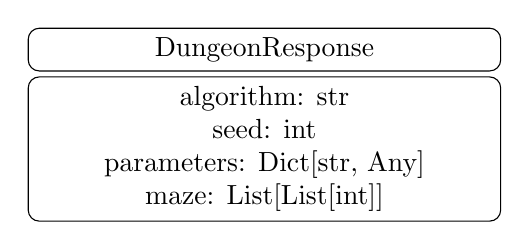
\begin{tikzpicture}
     \tikzstyle{every node}=[draw, shape=rectangle, rounded corners, align=center, minimum width=6cm]
     \node (dr) {DungeonResponse};
     \node[below, yshift=-0.34cm] (fields) {algorithm: str\\ seed: int\\ parameters: Dict[str, Any]\\ maze: List[List[int]]};
 \end{tikzpicture}
 \caption{Diagrama del nodo DungeonResponse}
 \end{figure}


\subsection{Ventajas del diseño NoSQL}

El uso de una base de datos NoSQL, específicamente MongoDB, proporciona diversas ventajas en este contexto, a saber:

\begin{itemize}
    \item \textbf{Flexibilidad en el esquema}. La estructura flexible de documentos en MongoDB permite modificar el modelo de datos sin necesidad de migraciones complejas.
    \item \textbf{Escalabilidad}. MongoDB está diseñado para manejar grandes volúmenes de datos y proporciona escalabilidad horizontal mediante la partición de datos (\textit{sharding}).
    \item \textbf{Consultas rápidas}. Las consultas y agregaciones en MongoDB son rápidas y eficientes, lo cual es crucial para aplicaciones que requieren respuestas en tiempo real.
\end{itemize}


\section{Diseño procedimental}
En esta sección se describen los procedimientos utilizados en el proyecto para controlar el flujo de información que hay entre el usuario y el proyecto. Para poder ilustrarlos, se diseñan varios diagramas de secuencia siguiendo la normativa UML. 

En primer lugar, se va a analizar el flujo de información que se da cuando se genera un laberinto nuevo; es decir, cuando el laberinto no está inicialmente almacenado en la base de datos del servidor. Corresponde con la figura \ref{fig:LaberintoNuevo}.

En segundo lugar, se va a analizar el caso en el que el laberinto sí se encuentra ya generado en la base de datos. Corresponde con la figura \ref{fig:LaberintoAlmacenado}.

\begin{figure}[H]
    \centering  
    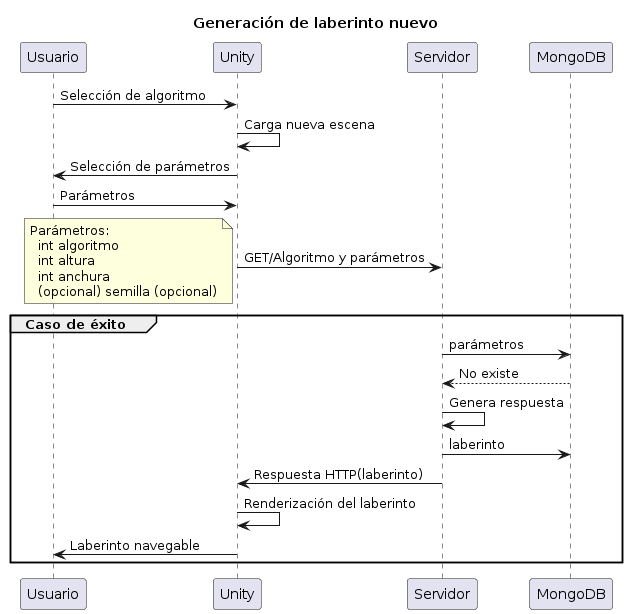
\includegraphics[width=\textwidth]{img/LaberintoNuevo.png}  
    \caption{Diagrama de secuencias de un laberinto nuevo.}  
    \label{fig:LaberintoNuevo}
\end{figure}

\begin{figure}[H]
    \centering  
    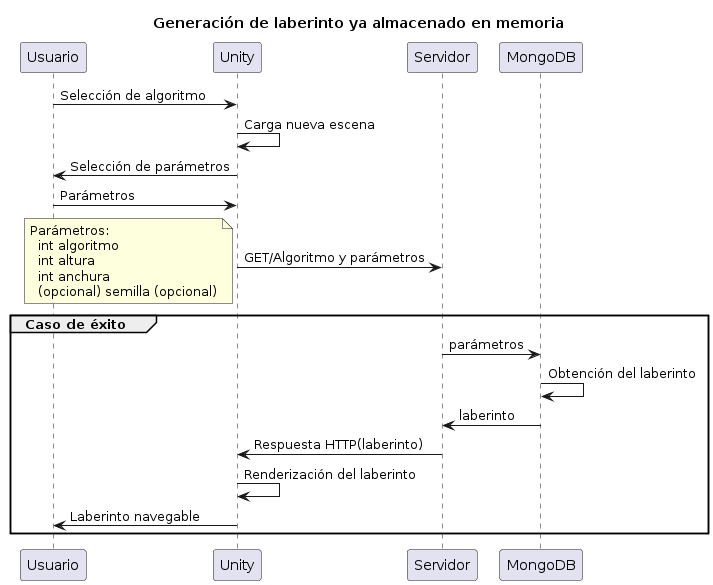
\includegraphics[width=\textwidth]{img/LaberintoYaAlmacenado.png}  
    \caption{Diagrama de secuencias de un laberinto ya almacenado.}  
    \label{fig:LaberintoAlmacenado}
\end{figure}



\section{Diseño arquitectónico}

El diseño arquitectónico de la aplicación se basa en una arquitectura cliente-servidor, donde el cliente está desarrollado en Unity, el servidor utiliza FastAPI y la base de datos es MongoDB. Este enfoque permite una comunicación eficiente y estructurada entre los componentes, asegurando un flujo de datos coherente y una gestión centralizada de la lógica de negocio. 

\subsection{Arquitectura cliente-servidor}

La arquitectura cliente-servidor empleada se divide en dos componentes principales:

\begin{itemize}
    \item \textbf{Cliente}. La interfaz gráfica y la lógica de presentación de la aplicación se desarrollan en Unity. Este componente es responsable de interactuar con el usuario final y de enviar solicitudes al servidor.
    \item \textbf{Servidor}. Este componente maneja las solicitudes del cliente, procesa la lógica de negocio y realiza operaciones sobre la base de datos. FastAPI, un \textit{framework} web moderno y rápido para Python, se utiliza para construir las API que facilitan la comunicación entre el cliente y el servidor. Por otro lado, en el lado del servidor localizamos también la base de datos MongoDB, que se utiliza para almacenar de manera eficiente los datos necesarios para la aplicación.
\end{itemize}

Esta arquitectura vista en conjunto no es monolítica, pero si se miran por separado cliente y servidor, cada uno de ellos son dos monolitos.

A continuación, en la Figura \ref{fig:arquitectura}, se presenta un diagrama que ilustra la arquitectura cliente-servidor.

\begin{figure}[!h]
    \centering
    \includegraphics[width=0.75\textwidth]{img/cliente_servidor.png}
    \caption[Arquitectura cliente-servidor.]{Arquitectura cliente-servidor\protect\footnotemark.}
    \label{fig:arquitectura}
\end{figure}

\footnotetext{Diagrama creado empleando iconos vectoriales de libre acceso desde la página \url{https://www.flaticon.es/}}

\subsection{FastAPI y REST}

FastAPI es un \textit{framework} web moderno para Python que permite la creación rápida y eficiente de API RESTful. Este \textit{framework} es conocido por su alto rendimiento y facilidad de uso, permitiendo a los desarrolladores definir y gestionar \textit{endpoints} de manera declarativa.

\subsubsection{REST}

REST (Representational State Transfer) es un estilo arquitectónico para diseñar servicios web que utilizan HTTP como protocolo de comunicación. Los principios de REST incluyen:

\begin{itemize}
    \item \textbf{Statelessness}. Cada solicitud del cliente al servidor debe contener toda la información necesaria para entender y procesar la solicitud.
    \item \textbf{Resource-Based}. Los recursos (datos) son identificados por URLs y pueden ser manipulados usando los métodos HTTP estándar (GET, POST, PUT, DELETE).
    \item \textbf{Representation}. Los recursos son representados en formatos estándar como JSON o XML.
\end{itemize}

\subsubsection{OpenAPI y Swagger}

FastAPI soporta de manera nativa la generación de documentación OpenAPI y Swagger. OpenAPI es una especificación que define una forma estándar de describir y documentar las API RESTful. Swagger es un conjunto de herramientas para la creación de documentación interactiva de API basadas en la especificación OpenAPI.

FastAPI genera automáticamente la documentación de la API en formato OpenAPI, y proporciona una interfaz web interactiva mediante Swagger UI, donde los desarrolladores pueden explorar y probar los \textit{endpoints} de la API.

\vspace{1em}

\begin{figure}[H]
    \centering
    \includegraphics[width=0.75\linewidth]{img/tech_arch.png} % Ignorar error, no afecta
    \caption{Tecnologías empleadas en la arquitectura}
    \label{fig:enter-label}
\end{figure}


\subsection{Modelo-Vista-Controlador}

El patrón de diseño Modelo-Vista-Controlador (MVC) se utiliza para estructurar la aplicación de manera que se separen claramente los intereses de datos, interfaz de usuario y control de flujo~\cite{mvc}. Este patrón se implementa de la siguiente manera:

\begin{itemize}
    \item \textbf{Modelo}: representa los datos y la lógica de negocio de la aplicación. En este caso, incluye las clases y estructuras que interactúan con la base de datos MongoDB, como \texttt{DungeonResponse}.
    \item \textbf{Vista}: maneja la representación visual de los datos y la interacción con el usuario. Unity actúa como la vista en esta arquitectura, proporcionando una interfaz gráfica interactiva.
    \item \textbf{Controlador}: interpreta las entradas del usuario y las convierte en acciones sobre el modelo. FastAPI sirve como el controlador, gestionando las solicitudes del cliente, aplicando la lógica de negocio y respondiendo adecuadamente.
\end{itemize}

El siguiente diagrama muestra la implementación del patrón MVC en la arquitectura.

\vspace{1em}

\begin{figure}[H]
    \centering
    \begin{tikzpicture}[node distance=3cm, auto, every node/.style={align=center}]
    
        % Nodes
        \node[rectangle, draw, fill=green!30] (view) {Vista};
        
        \node[rectangle, draw, fill=yellow!30, right of=view, node distance=5cm] (model) {Modelo};
        \node at ($(model)+(1.5,0)$) {
\includegraphics[height=1cm]{img/bbdd.png}};
    
        
        \node[rectangle, draw, fill=orange!30, below of=view, node distance=5cm] (controller) {Controlador};
        
        \node[left of=view, node distance=4cm] (user){
\includegraphics[height=1cm]{img/avatar.png}};
    
        % Arrows
        \draw[->] (view) -- node[anchor=east] {Llama} (controller);
        \draw[->] (controller) -- node[anchor=west] {Manipula} (model);
        \draw[->] (model) -- node[anchor=south] {Dispara eventos} (view);
        \draw[->, dashed] (user) -- node[anchor=south] {Interacción} (view);
    \end{tikzpicture}

    \caption{Patrón Modelo-Vista-Controlador}
    \label{fig:mvc}
\end{figure}

\subsection{Estrategia y Método Plantilla}
En el diseño del servidor se utilizan los patrones de diseño Estrategia y Método Plantilla para mejorar tanto la modularidad como la reutilización del código. Estos patrones permiten definir algoritmos específicos de manera concreta, mientras que las partes comunes se establecen en una clase base, facilitando la extensión del diseño con nuevos algoritmos sin modificar el código existente.

El patrón de diseño Estrategia es un patrón de diseño de comportamiento que define una familia de algoritmos, hace que se coloque cada uno de estos algoritmos en una clase separada, es decir, se encapsulan, y se hacen intercambiables~\cite{strategyPattern}. 

El patrón de diseño Método Plantilla es un patrón de diseño de comportamiento, este define el esqueleto de un algoritmo en la superclase pero también permite que las subclases sobrescriban pasos del algoritmo sin cambiar su estructura~\cite{templateMethodPattern}.

En el caso de este proyecto, cada algoritmo de generación procedimental es una estrategia concreta, no se redefinen al completo si no que cada uno hace uso de las partes comunes que están definidas en la clase base y las partes específicas en las clases hijas. De esta forma se mejora la modularidad del código, se reutiliza y se reduce la duplicidad de código. 

Al hacer uso de estos patrones se favorece el principio SOLID Open-Closed. Este propicia la extensión del diseño con nuevos algoritmos sin necesidad de modificar el código existente, haciendo un diseño abierto para extensión pero cerrado para la modificación~\cite{solidOpenClosed}. También se ve favorecido el principio de sustitución de Liskov, este permite que cualquier algoritmo de una subclase pueda sustituir a otro de una superclase sin alterar el comportamiento del programa, así se garantiza que las estrategias sean consistentes~\cite{liskovSubstitutionPrinciple}.
